\section{Загальні принципи використання стилів оформлення у текстовому процесорі \LaTeX{}}
\subsection{Стилі у \LaTeX{}}
\subsubsection{Загальні положення}

Стилі допомагають встановлювати оформлення для обраних елементів тексту. Оформлення включає:
\begin{itemize}
\item гарнітуру, розмір та особливості напису шрифту;
\item параметри абзацу, такі як відступи, міжстрочний інтервал, положення на сторінці;
\item нумерація або маркування списків;
\item колір шрифту або фону;
\item та інше.
\end{itemize}

Можливо обійтися без стилів, але у цьому випадку усі параметри треба встановлювати вручну для кожного елементу тексту. Крім того, неможливо буде скористуватись засобами автоматичної обробки документу, наприклад, можливістю автоматичної генерації змісту документа. 

\subsubsection{Стилі що реалізовані у шаблоні}

Для реалізації вимог стандарта або застосовується призначений стиль (див. 1.1.3) або виконуються допоміжні дії по редагуванню документа (див. 2). Перелік стилів включає:
\begin{enumerate}
\item верхний колонтитул;
\item заголовок 1;
\item заголовок 2;
\item заголовок 3;
\item заголовок 4;
\item маркированный стандартный;
\item нижний колонтитул;
\item номер рисунка;
\item номер страницы;
\item номер таблицы;
\item нумерованный стандартный;
\item нумерованный развернутый;
\item обычный
\item рисунок;
\item содержание
\item структурная часть приложения
\item текст таблицы
\item формула без номера
\item формула с номером
\item формулы описание.
\end{enumerate}

\subsubsection{Місце управління вимогами в процесі розробки програмного
забезпечення}

Перелік пунктів стандарту, що можуть бути автоматично виконані призначенням відповідного стилю:
\begin{enumerate}
\item текст документа (п.4.3) реалізується стилем Обычный;
\item зміст (п.5.3) автоматично генерується на основі призначення стилів Заголовок 1-3, для заголовку змісту використовується стиль Содержание;
\item перелік джерел інформації (п.5.8) реалізується з використанням стилю нумерованный развернутый;
\item переліки (п.6.2.7-6.2.10) реалізуються стилями маркированный стандартный, нумерованный стандартный, нумерованный развернутый, при цьому:
\begin{itemize}
  \item стиль нумерованный развернутый використовується коли у пунктах (хоча би одному) більш ніж одне речення; при цьому перед переліком ставиться крапка, в кінці кожного пункту ставиться крапка;
  \item стиль нумерованный стандартный використовується коли у кожному пункті одне речення, при цьому в кінці кожного пункту ставиться крапка з   комою а кінці останнього пункту ставиться крапка;
  \item вкладений перелік з маркером та збільшеним відступом реалізується операцією збільшення відступу (увеличить отступ) для обраних пунктів;
\end{itemize}
\item заголовки структурних підрозділів (п.6.2.11-6.2.15) реалізуються стилями Заголовок 1-3;
\item розташування формул (пп.6.3.2.1-6.3.2.3) реалізуються стилями Формула без номера, Формула с номером;
\item пояснення позначень у формулах (п. 6.3.2.4) реалізуються стилем Формулы описание;
\item розташування номеру таблиці (пп. 6.3.3.2) реалізується стилем Номер таблицы;
\item розташування рисунку (п. 6.3.4.3) реалізується стилем Рисунок;
\item розташування номеру рисунку (п. 6.3.4.4) реалізується стилем Номер рисунка.
\end{enumerate}

Усі інші пункти стандарту виконуються автором самостійно. Приклади оформлення представлені у наступних розділах.

\subsection{На які пункти стандарту слід звертати увагу}

6.2.6
6.2.11

\section{Нотатки по практичному застосуванню шаблона}
\subsection{Оформлення списку джерел інформації}

Оформлення списку джерел інформації проводиться згідно ДСТУ ГОСТ 7.1:2006 «Бібліографічний запис, бібліографічний опис. Загальні вимоги та правила складання» []. Приклади оформлення джерел наведені у даному документі [-]

\subsection{Використання складних стилів}
\subsubsection{Загальні положення}

Деякі задачі оформлення вимагають використання або двох стилів або диференційного використання одного стилю

\subsubsection{Багаторівневі списки}

Для створення підлеглого маркірованого списку у нумерованому списку (нумерованный стандартный, нумерованный развернутый) треба 

\subsubsection{Опис формули}

Змінні що використані у формулі та не були описані до того у тексті повинні бути описані відразу після формули. Для опису може бути використаний стиль Формулы описание. У цьому випадку опис кожної змінної відокремлюється від попереднього розривом строки (комбінація клавіш Shift+Enter) як представлено на рисунку

\subsubsection{Оформлення ілюстрацій}

При оформленні ілюстрацій необхідно виконати наступні вимоги:
\begin{itemize}
\item зробити відступ у одну пусту строку перед рисунком та після номеру рисунку;
\item розмістити рисунок посередині сторінки по горизонталі без відступу;
\item після рисунку розмістити номер рисунку (з назвою, якщо потрібно) посередині сторінки по горизонталі без відступу;
\item якщо у рисунку є підрисунковий текст, він розміщується відразу після рисунку аналогічно номеру;
\item треба запобігти відокремленню підрисункового тексту та номеру від рисунку при розбитті на сторінки (опція «не отрывать от следующего» у властивостях абзацу).
\end{itemize}

Виконати усі ці вимоги можна, призначив стиль Рисунок самому рисунку та підрисунковому тексту а стиль Номер рисунка (слідує автоматично) номеру рисунку. Пусти строки до та після ілюстрації виконуються автором самостійно. Номери також присвоюються автором самостійно.

\subsubsection{Оформлення додатків}

При виконанні додатків треба коректно виконати заголовок та при необхідності розбити додаток на структурні підрозділи. Заголовок додатку виконується за допомогою стилю Заголовок 1 з примусовим розбиттям на строки за допомогою комбінації клавіш Shift+Enter, як показано на рисунку:

Структурні підрозділи додатку оформлюються за допомогою стилю структурная часть приложения, відступи на нумерація виконуються автором самостійно. Заголовки, виконані таким чином не попадають у зміст документа, але на них можна робити посилання тексті.

\subsection{Переліки з позначеннями малими літерами української абетки}

Такі переліки повинні виключати літери є, з, і, ї, й, о, ч, ь тому ъх потрібно робити вручну та використовувати стиль Обычный.

\subsection{Робота зі стилями}

Стилі зберігаються у файлі з роботою. При необхідності вони можуть експортуватися із файлу шаблону. Призначення стилю даному абзацу перевизначає параметри шрифту, абзацу, нумерації та інші. Для цього можна імпортувати стилі із шаблону (Шаблоны и настройки) та встановити параметр Автоматически обновлять стили. Стилі додаються, редагуються та видаляються зі списку стилів. Також можна виділити весь текст що має заданий стиль, наприклад, щоб назначити інший стиль. 

Для того щоб робота зі стилями була більш ефективною рекомендується виконувати титульні листи в окремому документі, тому що їх оформлення вимагає більшої кількості нестандартних стилів.

\subsection{Можливі проблеми та підходи до їх розв’язання}

Проблеми використання розробленого шаблону мають різне походження, у переліку представлені найбільш поширені.
\begin{enumerate}
\item При розривах розділу, наприклад, для вставки сторінок у альбомній орієнтації, може стати некоректною нумерація сторінок після розділу. Можна досягнути коректності нумерації налаштуванням розділів та нумерації. Можна оставити пусти сторінки для великих ілюстрацій які розробити у зовнішніх документах а потім друкувати їх на пустих сторінках з надрукованими номерами сторінок.
\item Нумерація нумерованих переліків може починатись не з одиниці а з іншого числа. Треба кликнути правою кнопку миші кликнути на номері верхнього пункту та обрати Начать заново. Якщо проблема залишилася (наприклад, перший пункт має номер 1, а починаючи з другого продовжується інша нумерація) треба виділити всі пункти переліку, обрати стиль Очистить формат далі обрати стиль Обычный а потім знову обрати стиль потрібного переліку.
\item Під’єднання шаблону може складним чином взаємодіяти зі стилями документу та не давати того результату що очікується. При наявності готового тексту краще скопіювати текст та вставити в документ що розданий на основі шаблону, а далі застосувати належні стилі до елементів тексту.
\item Опис формули (стиль ) може некоректно відображати змінні що побудовані як формула (MS Equation) що відбивається в тому що відступ нової строки не відбивається. У цьому випадку треба або поставити пробіл перед позначенням змінним або використаи звичайний стиль та зробити відступи вручну. 
\end{enumerate}

\section{Приклади використання стилів}

\subsection{Огляд методів моделювання й опису процесів}
\subsubsection{Загальні положення}
Моделі виробничих процесів можна класифікувати в наступному виді []:
\begin{itemize}
\item описові;
\item алгоритмічні;
\item математичні;
\item \dots~.
\end{itemize}

Математичні моделі ...

\subsubsection{Методи імітаційного моделювання}
Імітаційна модель~-- це математична модель, що відбиває істотні для дослідника особливості досліджуваної системи.

Імітаційні моделі створюються для рішення наступних завдань:
\begin{enumerate}
\item визначення реакції складної системи на керуючий вплив у ситуації, коли безпосередні експерименти з нею дорогі, складні, або небезпечні;
\item \dots
\item в інших ситуаціях, що вимагають попередньої оцінки наслідків прийнятих
рішень\footnote{Розглядається множина що … Розглядається множина що
Розглядається множина що Розглядається множина що Розглядається множина що
Розглядається множина що}:
\begin{itemize}
\item перша ситуація;
\item інша ситуація.
\end{itemize}
\end{enumerate}
У цей час використаються наступні інструментальні засоби імітаційного моделювання.
\begin{enumerate}
\item Система імітаційного моделювання GPSS. Це потужне середовище комп'ютерного моделювання загального призначення, розроблене для професіоналів в області моделювання. 
\item Це комплексний моделюючий інструмент, що охоплює області як дискретного, так і безперервного комп'ютерного моделювання, що має високий рівень інтерактивності й візуального подання інформації.
\item Пакет прикладних програм MATLAB. Призначений для рішення завдань технічних обчислень. Включає мову програмування. Використається більш ніж 1000000 інженерних і науковців, і працює на більшості сучасних операційних систем, включаючи:
\begin{itemize}
\item Linux; 
\item Mac OS; 
\item Solaris; 
\item Windows.
\end{itemize}
\item Система ARENA компанії Systems Modeling. Дозволяє будувати імітаційні моделі, програвати їх і аналізувати результати такого програвання, і ін.
\end{enumerate}

\subsubsection{Мова специфікації процесів (Process Specification Language)}
[текст пункту]
\subsubsection{Методологія IDEF}
Методологія IDEF (I-CAM DEFinition) розробляється компанією Knowledge Based Systems, Inc…
Стандарт IDEF0 призначений для моделювання
бізнес-функцій~\cite{Sommerville_2010}. Структура функціонального блока в методології IDEF0 приведена на рисунку
\ref{idef_fb}.

\begin{stdfigure}
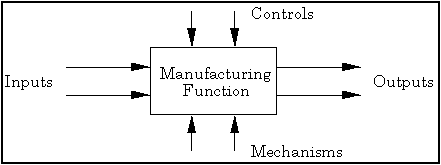
\includegraphics[width=2.7in]{images/idef_fb.png}
\caption{Структура функціонального блоку}
\label{idef_fb}
\end{stdfigure}

\subsection{Функціональний аналіз виробничого процесу зборки регулятора напруги}

Виробничий процес зборки регулятора напруги…

\subsection{Постановка задачі моделювання виробничого процесу зборки регулятора
напруги}

Необхідно розробити імітаційну модель процесу зборки регулятора напруги…

Моделі виробничих процесів можна класифікувати в наступному виді:
\begin{itemize}
\item описові;
\item алгоритмічні;
\item математичні.
\end{itemize}

Математичні моделі [текст пункту]


\subsection{Застосування мереж Петрі до вирішення задачі моделювання
виробничого процесу зборки регулятора напруги} 

…

Мережа Петрі $M = (C, \mu)$ є такою що строго зберігає, коли для всіх маркувань
$\mu' \in R(C, \mu)$ виконується співвідношення

\begin{equation}
\sum_{p_i \in P}{\mu'(p_i)}=\sum_{p_i \in P}{\mu(p_i)}
\end{equation}

\begin{formulaDescription}
\item[$\mu'$] маркування;
\item[$p_i$] перехід мережи.
\end{formulaDescription}

Таким чином, загальна кількість фішок в будь-якому маркуванні із множини
досяжності $R(C, \mu)$ дорівнює загальному числу фішок у початковому маркуванні
$\mu$.

…

Матричне подання мережі Петрі визначає іншу форму основних правил виконання
мережі - правила дозволу переходів і правила зміни маркування. Перехід $t_j \in 
T$ є дозволеним у маркуванні $\mu$, якщо виконується у векторному змісті
співвідношення

\begin{equation}\label{eqn:ejd}
\mu \geq e[j] D
\end{equation}

Оскільки $e[3] D^{-}$ = (0 0 1 0), то співвідношення (\ref{eqn:ejd}) виконується
для переходу t3 $\mu > e[3] D^{-}$. Отже, перехід t3 є дозволеним в
маркуванні $\mu = ( 1 0 1 0 )$.

…

\subsection{Функціональна структура програмного забезпечення із застосуванням
IDEF0-методології}

…

\subsection{Інформаційно-логічна схема програмного забезпечення із застосуванням
IDEF1Х-методологии}

…

\subsection{Посібник користувача програмного забезпечення}

…

\section{Застосування розробленого програмного забезпечення до моделювання
виробничого процесу зборки регулятора напруги}

\subsection{Вхідна й вихідна інформація}

Технологічні характеристики встаткування наведені в додатку А. 

…

На рисунку 4.1 наведено алгоритм обчислення характеристик обладнання.

\subsection{Аналіз отриманих результатів моделювання}
\begin{longtable}{5}{|m{2cm}|m{3cm}|m{3cm}|m{3cm}|m{2cm}|}
{\label{tbl:experiment}Результати
проведення чисельних експериментів з математичною моделлю}
{  
 № варіанта &
\multicolumn{3}{l|}{Значення параметрів технологічного встаткування} &
Час зборки, с \\ \cline{2-4}
& A & B & C &
}

1 & & & & \\ \hline
2 & & & & \\ \hline 
3 & & & & \\ \hline
4 & & & & \\ \hline
5 & & & & \\ \hline
6 & & & & \\ \hline
7 & & & & \\ \hline
8 & & & & \\ \hline
9 & & & & \\ \hline
10 & & & & \\ \hline
11 & & & & \\ \hline
12 & & & & \\ \hline
13 & & & & \\ \hline
15 & & & & \\ \hline
16 & & & & \\ \hline
17 & & & & \\ \hline
18 & & & & \\ \hline
19 & & & & \\ \hline
20 & & & & \\ \hline
21 & & & & \\ \hline
22 & & & & \\ \hline
23 & & & & \\ \hline
24 & & & & \\ \hline
25 & & & & \\ \hline
26 & & & & \\ \hline
27 & & & & \\ \hline
\end{longtable}

Результати моделювання наведені в таблиці \ref{tbl:experiment}.

\begin{shorttable}{2}{|c|c|}
{\label{tbl:ndrparam}Характеристика роботи}
{
Час спостережень &
Значення параметру
}
00:01 & 1 \\ \hline
00:02 & 2 \\ \hline
00:03 & 1 \\ \hline
00:04 & 3 \\ \hline
\end{shorttable}

